\section{Proposed Algorithm} \label{sec:algorithm}

\subsection{Naive Trie-Building Algorithm} \label{sec:algorithm:naive}

The existing algorithm functions by treating the ordered rank-differentia pairs as strings (with potential missing information), where each differentia could represent a character at the rank-th position (recall that a \textit{rank} refers to a specific generation, and a \textit{differentia} refers to information retained at that generation).
With this abstraction, we can essentially build a trie \citep{fredkin1960trie} from the organisms, which is a data structure in which each path along the tree represents a string formed by the characters at each node along that path.

To begin, all organisms are sorted in ascending order by the number of generations elapsed; due to each organism using the same algorithm to determine which data to remove, if data at some rank is missing in one organism, it will be missing in all subsequent ones.
This list of organisms is then processed one at a time, going through each rank-differentia pair and determining whether to branch off the trie, continue along, or address missing information (see Algorithm~\ref{alg:old}).

\begin{algorithm}[h]
    \caption{the existing algorithm for creating a phylogenetic tree through hereditary stratigraphy, using a naive trie-building approach}
    \label{alg:old}
    \begin{algorithmic}[1]
        \Require a list of organisms $O$ in ascending order by generations elapsed
        \Function{ReconstructTree}{$O$}
            \State $T \gets$ an empty tree
            \For {$o \in O$} 
                \State $\textsc{TreeInsert}(T, o)$
            \EndFor
            \State \Return $T$
        \EndFunction

        \Function{TreeInsert}{$T, o$}
            \State $n \gets$ root of $T$
            \For{each rank-differentia pair $(r, d) \in o$}
                \While{$r >$ the rank of $n$'s children}
                    \State $n \gets$ the child of $n$ most likely contain $o$
                \EndWhile
                \If{$\exists c \in \operatorname{children}(n) \text{ s.t.} \operatorname{differentia(c) = d}$}
                    \State $n \gets c$
                \Else 
                    \State create a new child $c'$ branching off $n$ 
                    \State $\operatorname{differentia}(c') \gets d$
                    \State $n \gets c'$
                \EndIf
            \EndFor
            \State insert information about $o$ as a child of $n$
        \EndFunction
    \end{algorithmic}
\end{algorithm}

If processing information corresponding to a rank $r$ that is larger than the rank $r'$ of a child $c$ of $n$, we know that the information at rank $r'$ must have been deleted in the original organism (otherwise, it would have been processed already).
To maximize reconstruction accuracy, we must deterrmine if the missing datum is child $c$'s differentia, that of another child also with rank $r'$, or by none of the children of $n$ (where we would branch off).
Essentially, when reaching missing information, we must infer that information, which we do by looking ahead on the tree. The naive  trie algorithm accomplished this by looking forwards and finding the path with the ``longest successive streak'' of matching differentia with the current organism \citep{moreno2024analysis}.
If there is no matching path, we simply branch off $n$ rather than through its children.

However, despite being an accurate way of dealing with missing information, this approach suffers the cost of doing significant extra work each time.
In the worst case, there could be many matching paths to check, each with many matching differentiae.
In large-scale simulations, with limited differentia values (sometimes being represented with only one bit), this is a surprisingly common problem and significantly slows down the reconstruction process.
Additionally, these searches would need to happen for each organism, regardless of whether or not a similar search was already done.
Therefore, we present an improved algorithm that consolidates this extra work into a single step, never needing to be repeated.

\subsection{Proposed Shortcut Algorithm} \label{sec:algorithm:shortcut}

We present a modification of Algorithm~\ref{alg:old} where we replace the best path search in line 9 with a more intelligent consolidation step to deal with missing ranks. The main idea of this algorithm is to realize that, as previously stated, once data from a specific rank is no longer included in one organism, it will not be included in any subsequent organisms, meaning that the nodes in the tree corresponding to that rank are no longer useful. So, by building shortcuts around any nodes that were made irrelevant, we can speed up the reconstruction process for all future nodes too.

We detect missing information the same way as in the naive trie algorithm: during iteration, we notice that when a child $c$ of the current node $n$ has a rank $r'$ that is less than the current rank $r$ being processed, we do not have information about that rank. The key insight to the way we manage this is that, in the big picture, we only care about this child if some of its descendants at rank $r$ have the differentia equal to $d$. Also, since every subsequent organism does not contain information at rank $r'$ (due to the sorting), this statement holds throughout the rest of the algorithm.

\begin{figure*}
\begin{minipage}{0.74\linewidth}
\centering
\begin{minipage}{0.32\linewidth}
  \centering
  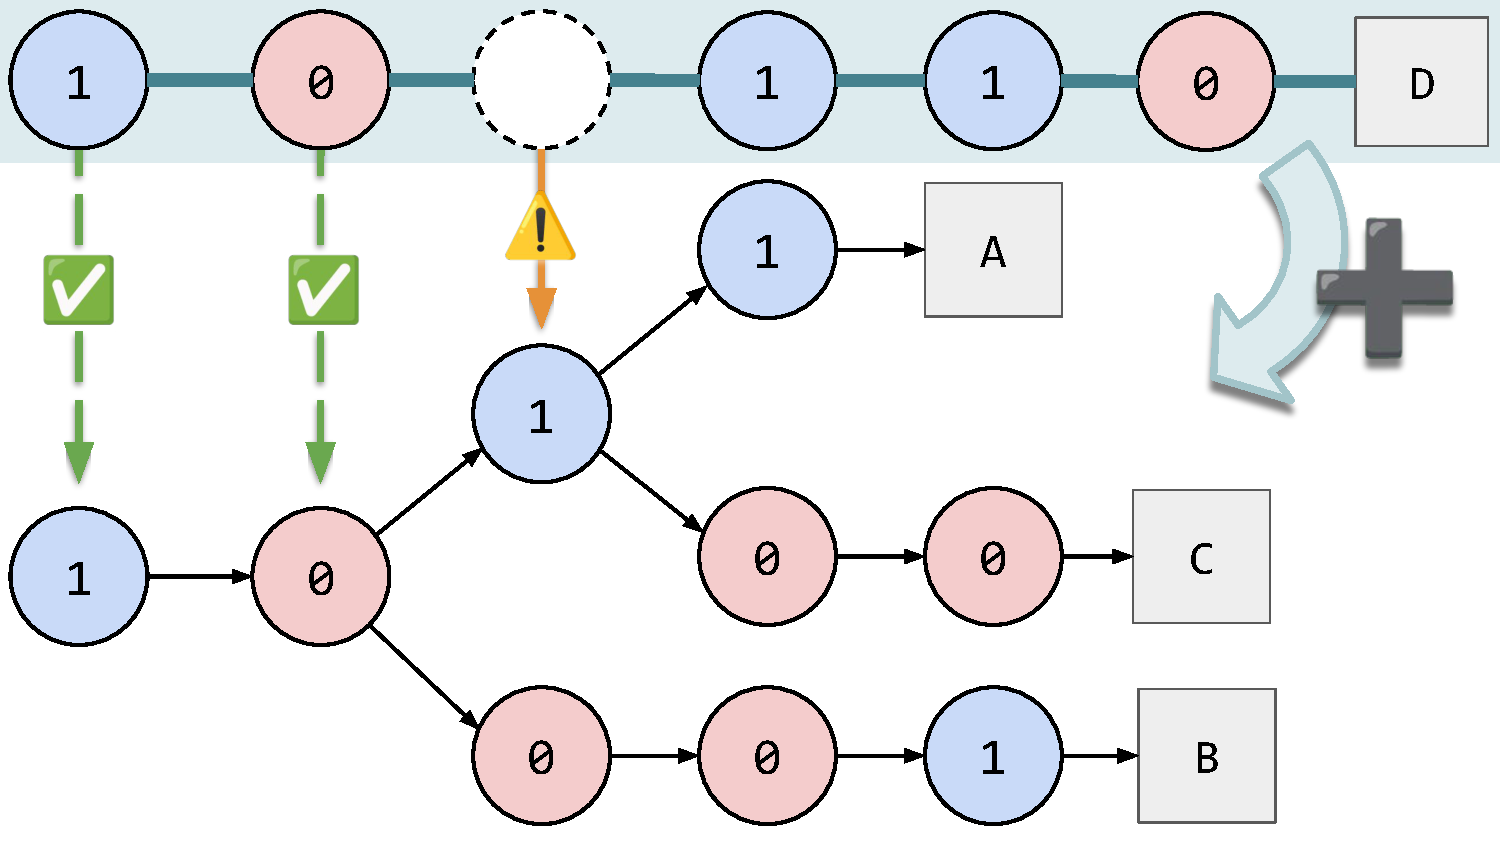
\includegraphics[width=\linewidth]{img/shortcut-algo-diagram-1}
  \subcaption{Preparing to add $D$}
  \label{fig:shortcut-algo-diagram-1}
\end{minipage}
\begin{minipage}{0.32\linewidth}
  \centering
  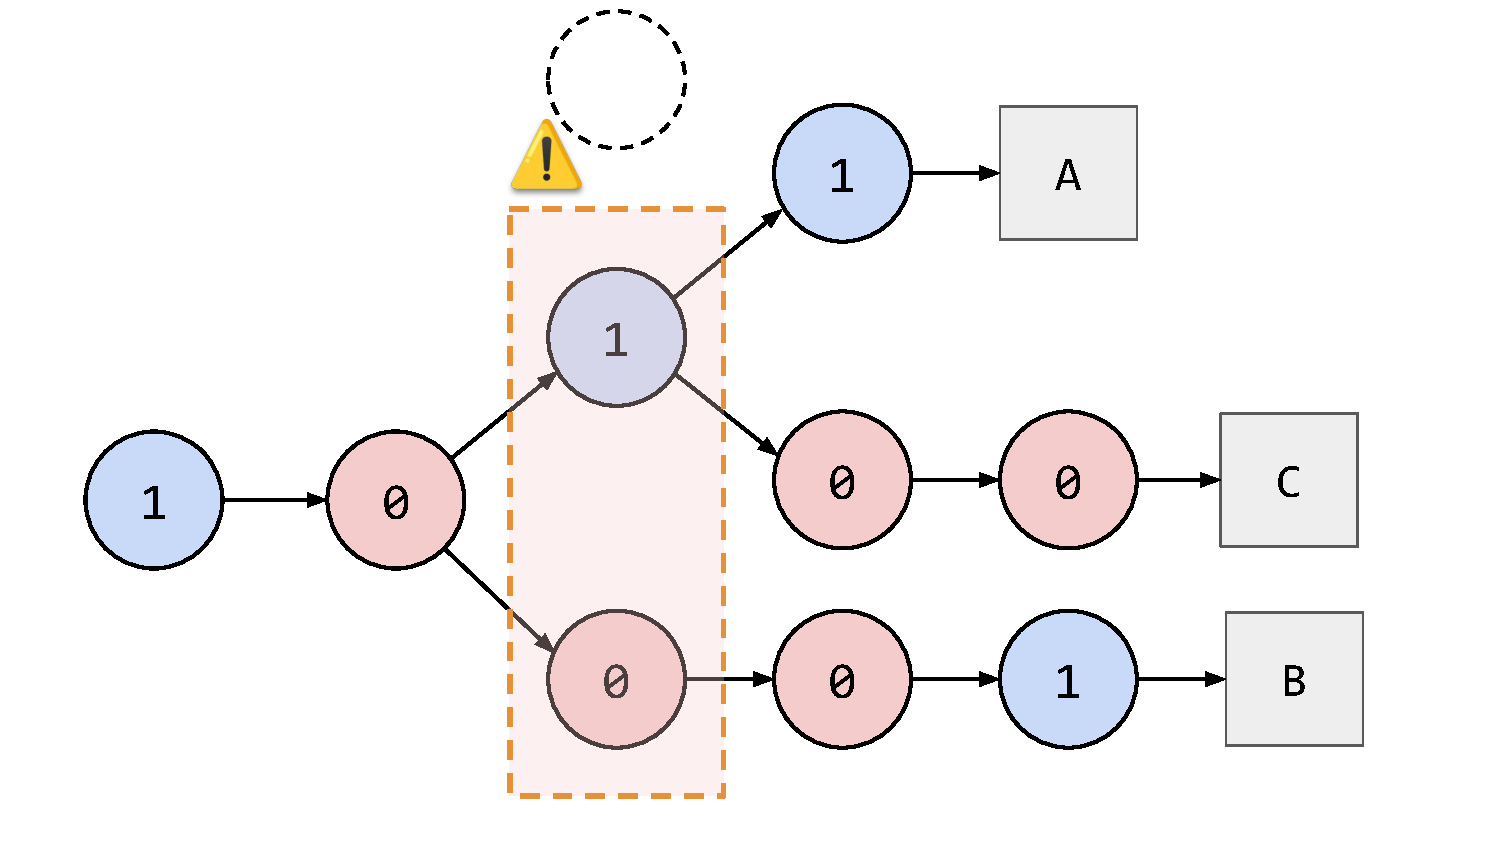
\includegraphics[width=\linewidth]{img/shortcut-algo-diagram-2}
  \subcaption{Encountering dropped marker}
  \label{fig:shortcut-algo-diagram-2}
\end{minipage}
\begin{minipage}{0.32\linewidth}
  \centering
  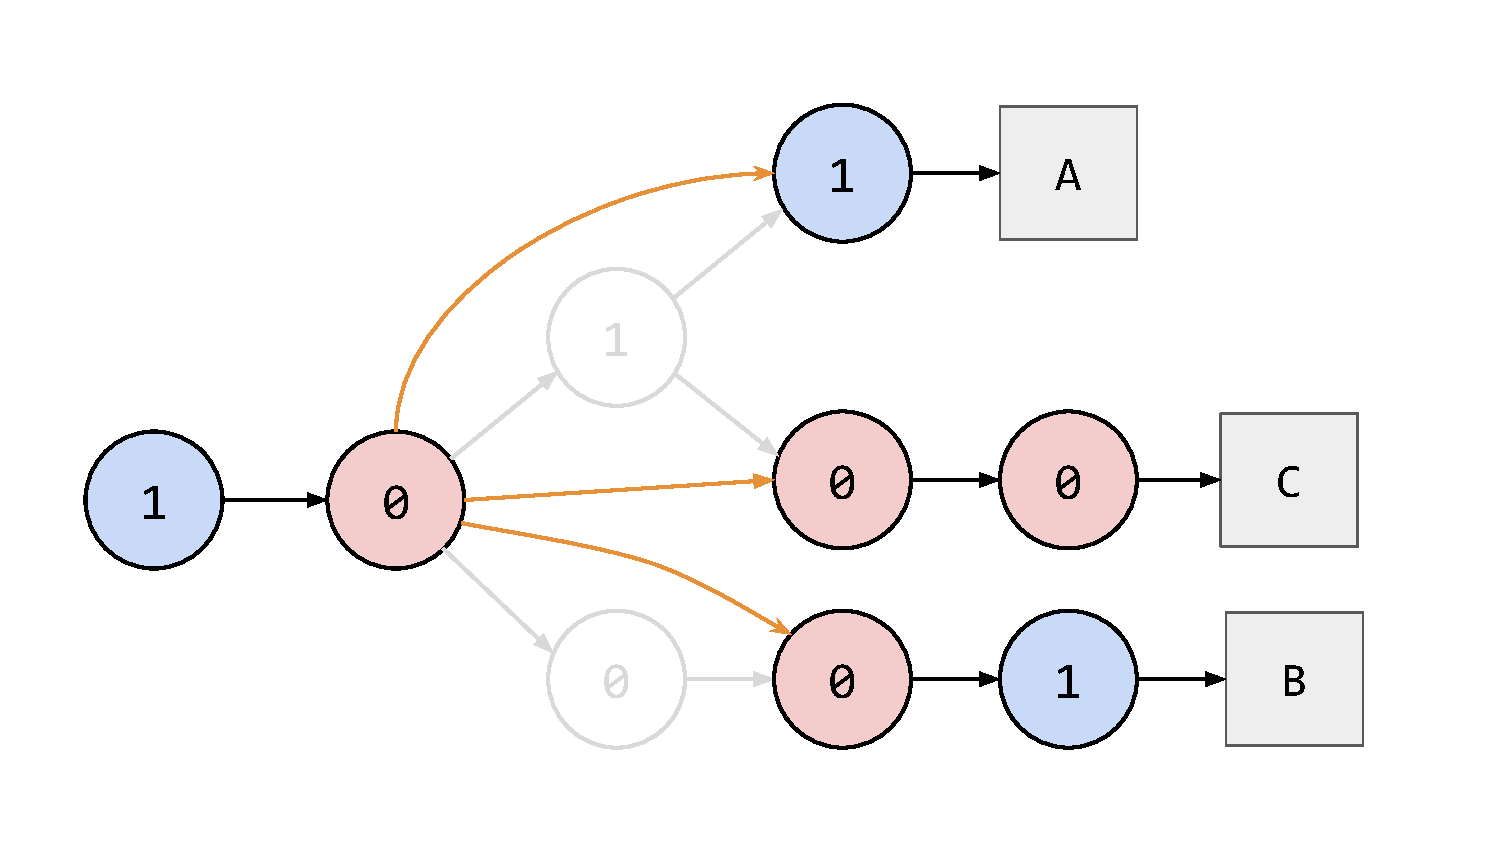
\includegraphics[width=\linewidth]{img/shortcut-algo-diagram-3}
  \subcaption{Building shortcuts}
  \label{fig:shortcut-algo-diagram-3}
\end{minipage}
\begin{minipage}{\linewidth}\par\end{minipage}
\begin{minipage}{0.32\linewidth}
  \centering
  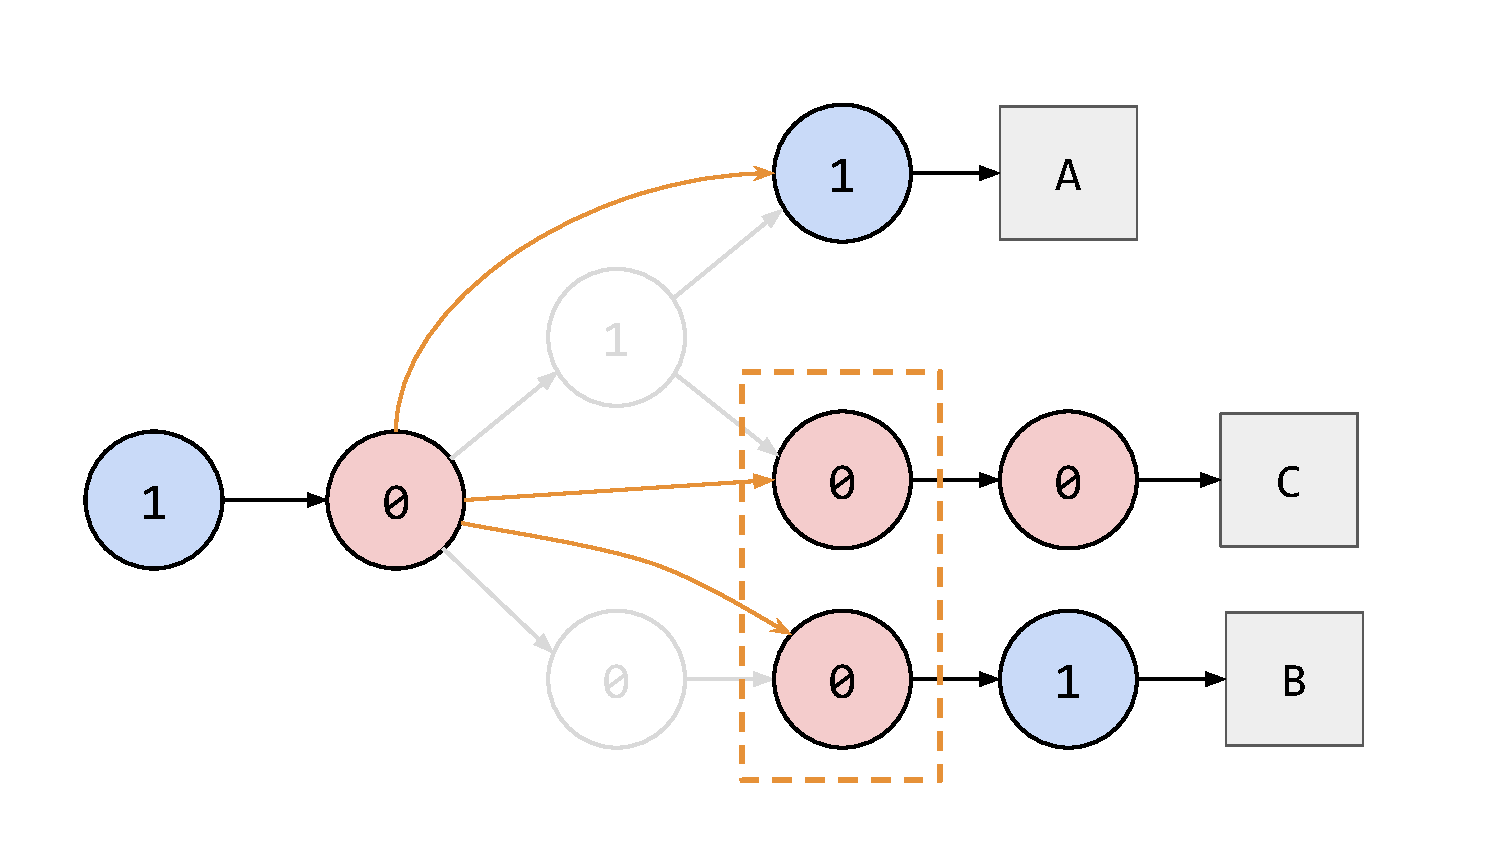
\includegraphics[width=\linewidth]{img/shortcut-algo-diagram-4}
  \subcaption{Indistinguishable nodes}
  \label{fig:shortcut-algo-diagram-4}
\end{minipage}
\begin{minipage}{0.32\linewidth}
  \centering
  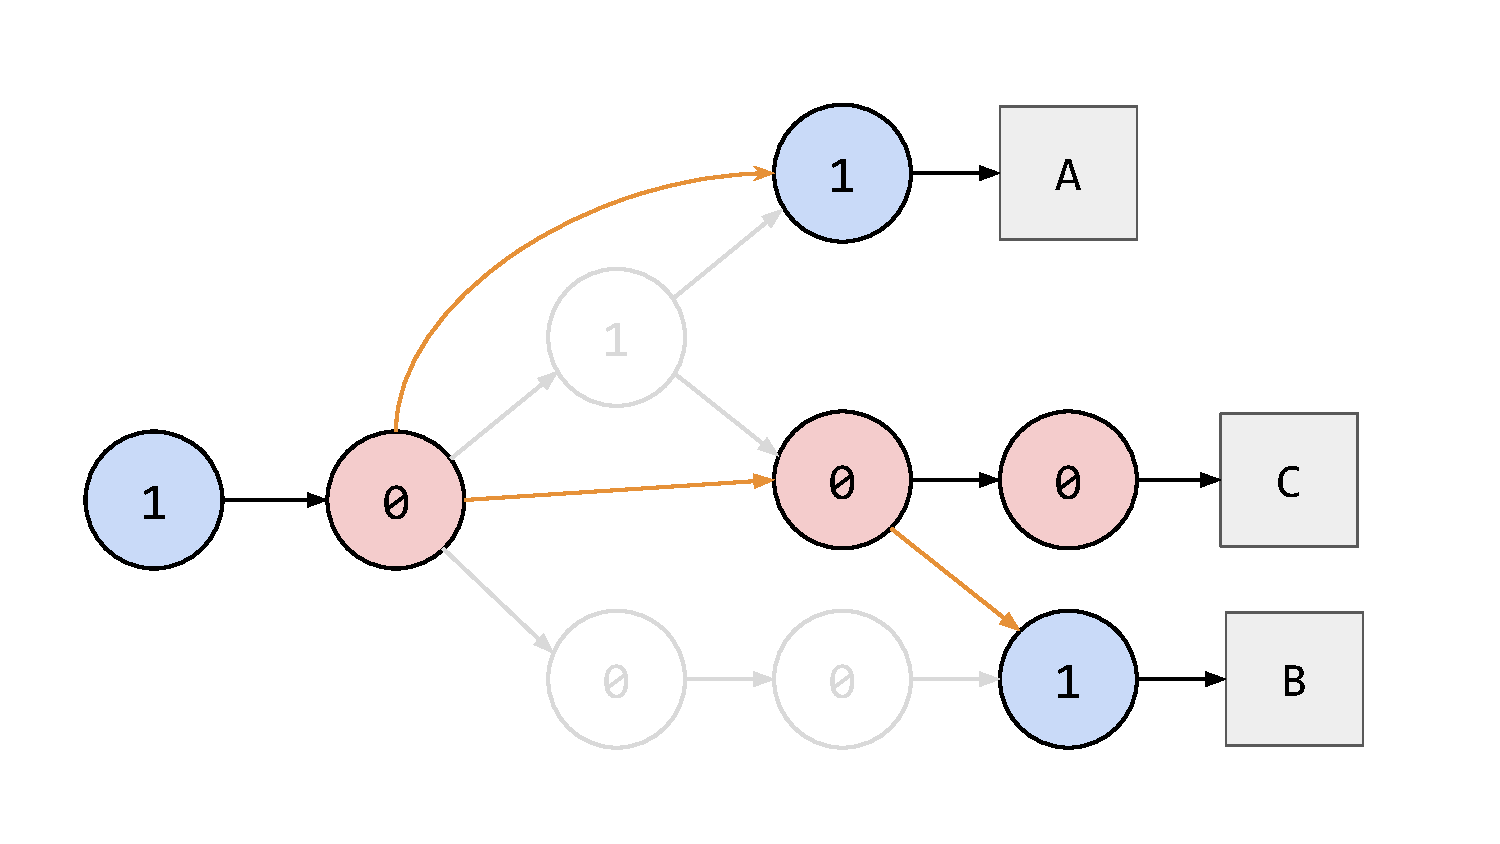
\includegraphics[width=\linewidth]{img/shortcut-algo-diagram-5}
  \subcaption{Collapsing redundant shortcuts}
  \label{fig:shortcut-algo-diagram-5}
\end{minipage}
\begin{minipage}{0.32\linewidth}
  \centering
  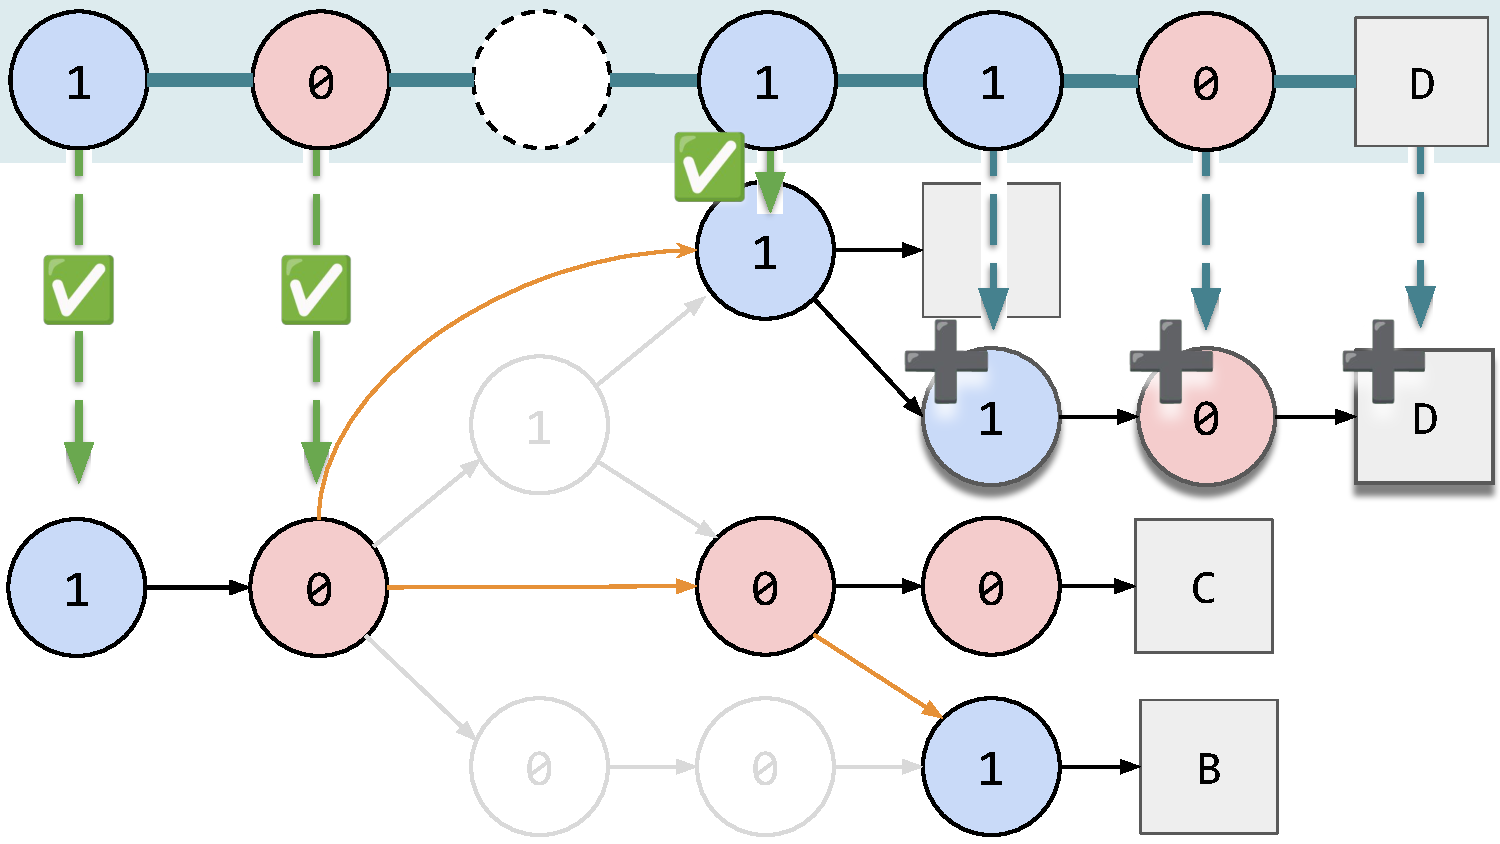
\includegraphics[width=\linewidth]{img/shortcut-algo-diagram-6}
  \subcaption{Organism $D$ added}
  \label{fig:shortcut-algo-diagram-6}
\end{minipage}
\end{minipage}
\begin{minipage}{0.24\linewidth}
\caption{%
\textbf{Trie-consolidation procedure for proposed shortcut algorithm.}
\small
A dropped hereditary marker is encountered while extending trie with genome $D$ (panel \ref{fig:shortcut-algo-diagram-2}).
All subsequent-added genomes will also have dropped markers at this position, so corresponding trie nodes may be bypassed by ``shortcut'' connections (panel \ref{fig:shortcut-algo-diagram-3}).
Note that bypassed trie structure is retained (``grayed-out'' nodes), so corresponding phylogenetic structure remains when reconstruction is finalized.
In a final step, shortcuts leading to identical nodes are further consolidated (panels \ref{fig:shortcut-algo-diagram-4} and \ref{fig:shortcut-algo-diagram-5}).
}
\label{fig:algo-diagram}
\end{minipage}
\vspace{-1.5em}
\end{figure*}


Extending this idea, since we know that any rank between $r'$ and $r$ is meaningless (as they all must have been deleted organism $o$ and any subsequent organisms), we create shortcuts from $n$ that bypass every one of its descendants that have a rank less than $r$.
In other words, on every possible path down the tree starting from $n$, we build a shortcut from $n$ to the first node on the tree with a rank at least $r$. For an example of what this looks like, see steps (b) and (c) in Figure~\ref{fig:algo-diagram}.

However, since some descendants of $n$ may have children with equivalent information, we may end up with shortcuts from $n$ to effectively indistinguishable nodes (with different original parents but the same information).
This can be resolved by essentially `merging' the duplicates by choosing one to keep and creating shortcuts from the kept one to the children of the removed one (see steps (d) and (e) in Figure~\ref{fig:algo-diagram}).

Now, adding any organisms that are missing data from the removed level becomes trivial, as the algorithm can use the newly created shortcuts while skipping the missing information that was hidden by the consolidation step.
We no longer need to look down branches from $n$ because each child of $n$ now has a rank greater than or equal to $r$. So, there is no longer a concern of missing information when processing $n$ at rank $r$, and these shortcuts are then used to add any subsequent organisms if need be.
If, at some point in the algorithm, $r$ itself becomes a rank of missing information, additional shortcuts can be built.

\begin{algorithm}[h]
  \begin{algorithmic}[1]
  \small{
    \Function{ConsolidateTree}{tree $T$, node $n$, rank $r$}
      \State $S \gets \{c \in \operatorname{descendants}(n) : \operatorname{rank}(c) \ge r \land  \operatorname{rank}(\operatorname{parent}(c)) < r\}$ 
      \For{$c$ in $S$} 
        \textsc{BuildShortcut}($T$, $n$, $c$)
      \EndFor
      \For{each subset of duplicate\footnotemark nodes $S' \subseteq S$}
        \State $c^* \gets$ an arbitrary element in $S'$ 
        \For{$c' \in S \setminus \{c^*\}$}
          \For{$c$ in $\operatorname{children}(c)$} 
            \State \textsc{BuildShortcut}($T$, $c^*$, $c$)
          \EndFor
          \State \textsc{RemoveShortcut}($T$, $n$, $c'$)
        \EndFor
      \EndFor 
    \EndFunction
    \Function{BuildShortcut}{tree $T$, node $n$, node $c$}
      \State $\operatorname{edges}(T) \gets \operatorname{edges}(T) \cup \{(n, c)\}$
      \State $\operatorname{edges}(T)[(n, c)]\text{.is\_shortcut} \gets \textsc{True}$
    \EndFunction
    \Function{RemoveShortcut}{tree $T$, node $n$, node $c$}
        \State $\operatorname{edges}(T) \gets \operatorname{edges}(T) \setminus \{(n, c)\}$
    \EndFunction
  }
  \end{algorithmic}
  \caption{\textbf{The consolidation step of the shortcut table algorithm.} \small Builds shortcuts for a given node $n$ and collapses duplicate children caused by those shortcuts. Note that \vspace{-1.5em}}
  \label{alg:consolidation}
\end{algorithm}
\footnotetext{nodes $x$ and $y$ are duplicates iff $\operatorname{rank}(x) = \operatorname{rank}(y)$ and $\operatorname{differentia}(x) = \operatorname{differentia}(y)$}

The key part in maintaining accuracy lie in the fact that since retain the old information (as represented by the gray nodes in Figure~\ref{fig:algo-diagram}), we preserve the full detail and granularity of the old approach. After the algorithm is run, we can simply use the remaining old information as the main phylogenetic tree. See Algorithm~\ref{alg:consolidation} to see psuedocode for this algorithm.